% chap2.tex (Definitions)

\chapter{Customer Load Forecasting in Power Trading Agent Competition}

We cannot think of modern civilization without the existence of electricity. Across the globe, electricity generation companies are spending trillions of dollars every year to produce Terawatt-hours of electricity to keep the wheel of the civilization running \cite{electricityStats}. A major portion of the electricity is produced by burning coal and natural gas \cite{electricityStats}. Alone the electricity generation is responsible for more than 40\% of all the greenhouse gas emissions \cite{schreiber2009environmental}. Around 4 million customers were disconnected from electricity in blackouts during 2003 \cite{andersson2005causes}. Electricity generation companies need to accurately forecast electricity load demand to avoid negative impacts on the environment, economic loss, and blackouts \cite{lodhi2013impact, sanghvi1982economic}. The companies may improve their load forecasting methods by utilizing the wealth of electricity usage data of their customers. In my thesis, I propose a data driven electricity load forecasting system. The system was tested on a realistic, smart grid \cite{fang2012smart} simulation platform called the Power Trading Agent Competition (Power TAC) \cite{ketter2013power}. The proposed mechanism is capable of making demand forecasts about a novel customer using data of known customer.

\section{Smart Grid}

In a power grid, there are three subsystems: electricity generation, transmission, and distribution \cite{fang2012smart}. In a typical electricity generation subsystem, the generator rotates a turbine in a magnetic field which generates electricity. Usually, the turbine rotates using the power of kinetic energy of water falling over a waterfall, a river with strong current, or from the reaction in nuclear power plant, or energy produced from burning coal or natural gas. The energy generation system then transmits the electricity through a transmission grid and finally through the distribution grid. A traditional generation system is one way, meaning that electricity the flow occurs only from generation node to consumption locations, and there is a little capability to collect information and intelligently manage the grid at all levels. In Figure \ref{fig:tradgrid}, flow of electricity is shown by an arrow. It can be seen that all the arrows start from electricity generation and in the consumer's direction which indicates flow of electricity.

\begin{figure}[h]
  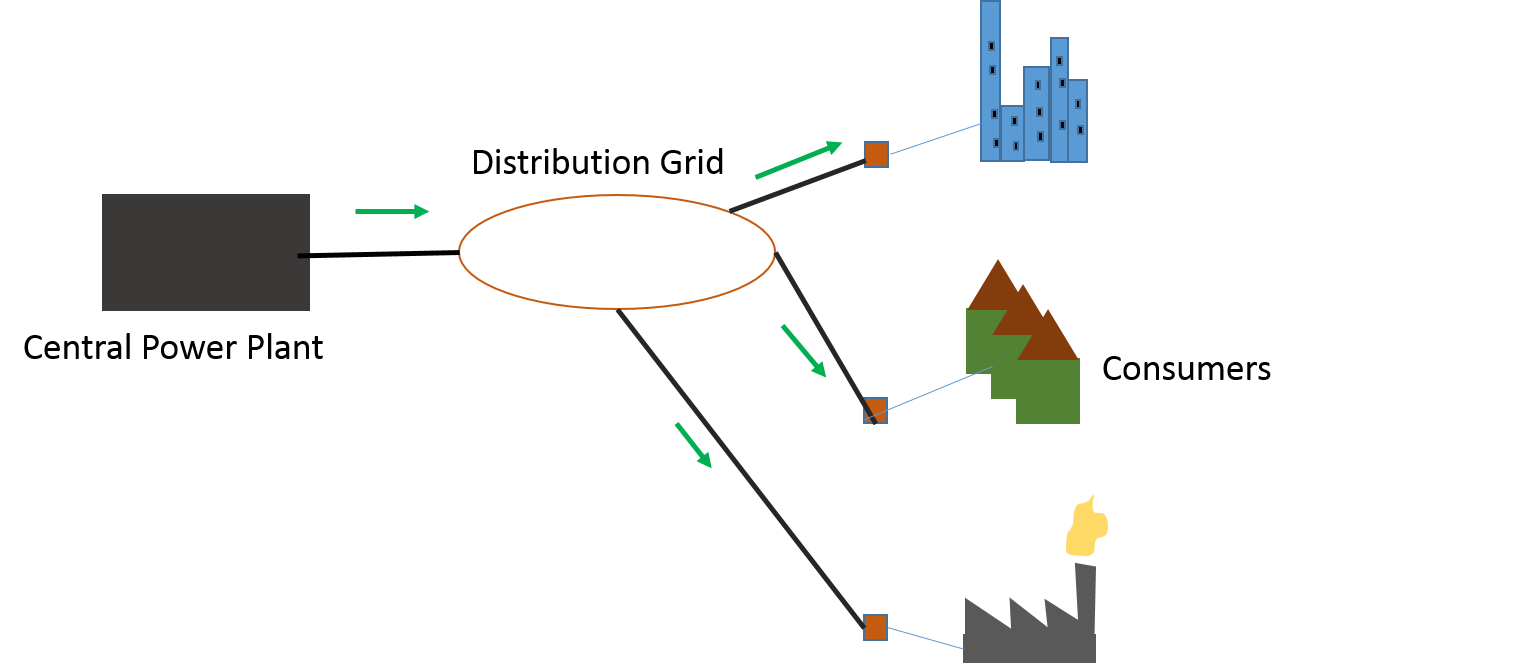
\includegraphics[width=\linewidth]{traditional.png}
  \caption{Traditional electricity generation and distribution system.}
  \label{fig:tradgrid}
\end{figure}

In contrast to the traditional electricity generation system, the Smart Grid (SG) is two-way \cite{fang2012smart}. Any node in the distribution grid can both consume and produce electricity to supply to the distribution grid. In Figure \ref{fig:smartgrid} a smart grid based electricity generation and distribution system are depicted. We can see that, in this system a flow toward the distribution system is possible. For example, renewable energy sources and household customers with solar energy production capabilities are pushing electricity to the power grid. The National Institute of Standards and Technology report states that the SG could make the electricity generation and supply robust against generator or distribution node failure, promote the use renewable energy, widely and efficiently, reduce greenhouse gas emissions, reduce oil consumption by encouraging usage of electric vehicles, and give customers more freedom to choose among energy sources. Smart grids will encourage usage of electric vehicles since these vehicles have the ability to store power in a battery and transmit the power to the distribution grid if there is a need \cite{fang2012smart}. Customers are showing strong motivation to use renewable energy as indicated by the statistics that 20\% of total energy is from the renewable sources which are second after coal 24\%. Consumers are using renewable energy due to economic reward and environmental concern. The major challenge with the usage of renewable energy as part of the supply is that it is uncertain \cite{richter2012transitioning}. This uncertainty causes problems for predicting how much energy the SG can produce in a future time slot. To manage the SG efficiently we will need effective methods to predict both energy production and load demand so they can be balanced in real time \cite{potter2009building}.

\begin{figure}[h]
  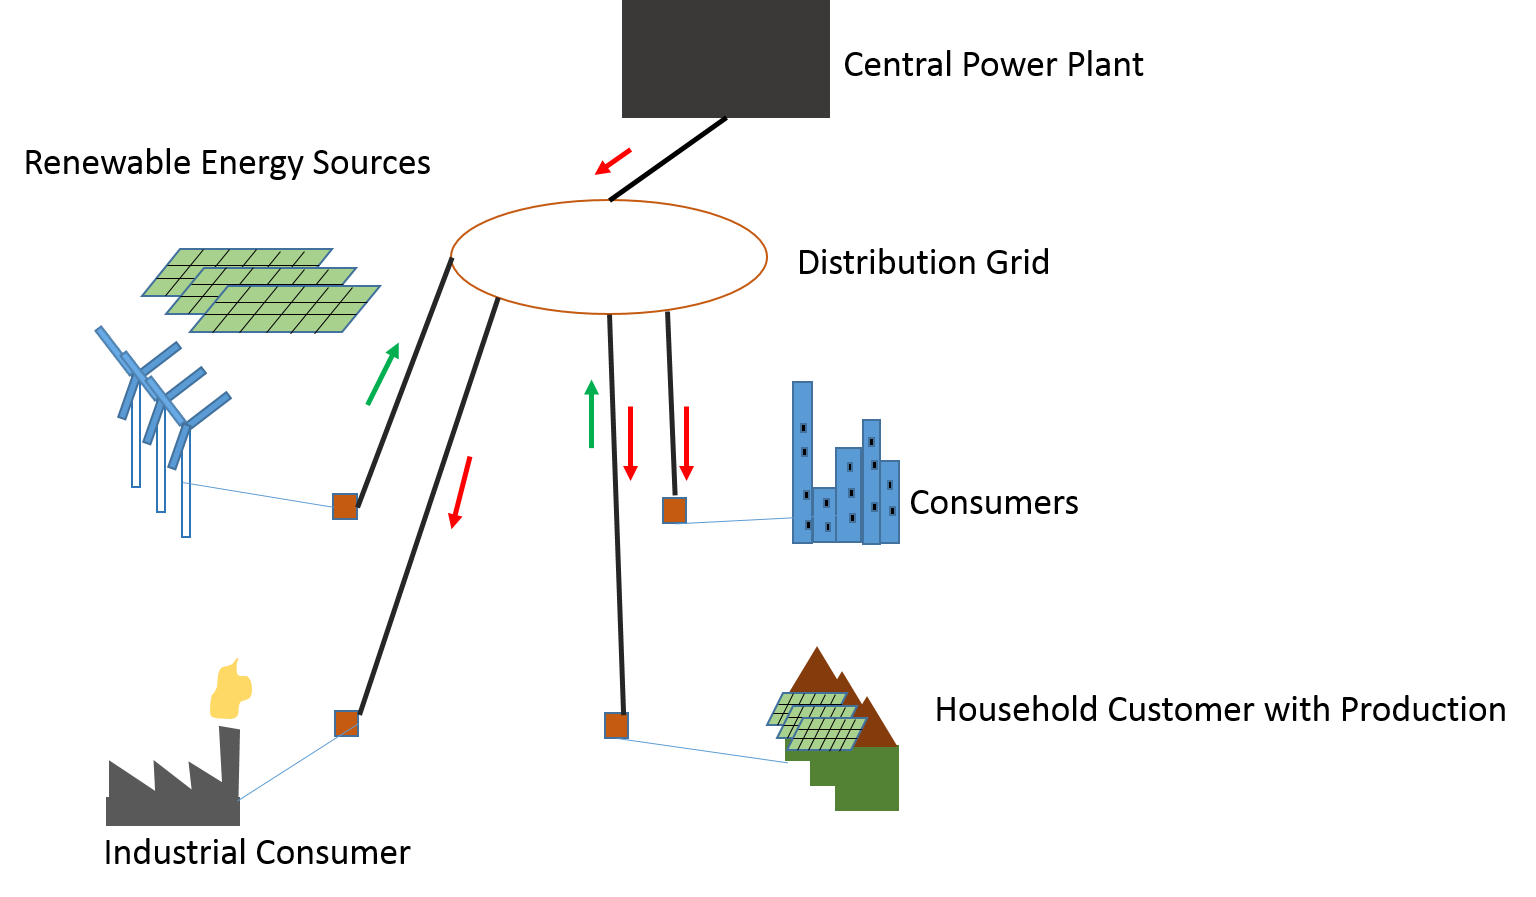
\includegraphics[width=\linewidth]{smart-grid.png}
  \caption{Smart grid based electricity generation and distribution system.}
  \label{fig:smartgrid}
\end{figure}

\section{The Power Trading Agent Competition}

The Power Trading Agent Competition (Power TAC), is an international research competition based on a smart grid energy market and distribution system \cite{ketter2013power, ketter20162016}. The Power TAC simulation models components including a wholesale market, electricity brokers, customers, a distribution utility and a weather service \cite{ketter20162016}. The brokers publish tariff plans for electricity consumers and producers. They buy electricity from the wholesale and balancing market to meet net customers demand. The system has realistic customer models and uses real weather data. Because of the realistic customer models present in the system, Power TAC can be used to do research on the customer electricity load demand. It is also useful because generating data is cheap in a computer simulation. The following sections give a brief explanation of each component of the Power TAC. Figure \ref{fig:simulation-environment}  shows a block diagram of the components of the Power TAC simulation environment.
%advantage 

\begin{figure}[!h]
  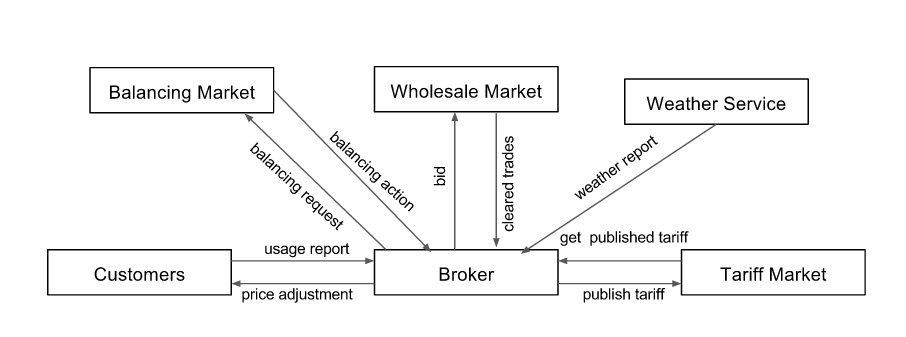
\includegraphics[width=\linewidth]{simulation-environment.png}
  \caption{Power TAC simulation environment.}
  \label{fig:simulation-environment}
\end{figure}

\subsection{Markets and Distribution Utility}

There are three different types of markets in the Power TAC simulation, namely, the wholesale market, tariff market and balancing market. The wholesale market is the bidding place for buying or selling energy. Bulk energy producers and brokers take part in the wholesale market auction. Brokers can submit their bids for 24 future timeslots in the wholesale market by specifying the price they are prepared to pay. If the bid was successful, the broker receives the desired quantity by paying the money. At each time slot, the system notifies the broker about the wholesale market clearing prices. Brokers publish their tariff plans in the tariff market. A tariff holds information about the pricing of the energy. Customers, upon analyzing available tariffs, subscribe to the most suited tariff plan. The balancing market represents the market from where the broker can buy energy in case of imbalance. For example, if a broker has bought less amount of energy for a given timeslot and it finds it needs more energy then it can buy the necessary amount of energy from the balancing market. Usually, the balancing market transactions are more costly for brokers than the wholesale market.

The distribution utility has two main objectives. First, it supplies energy to the consumers from the wholesale market and from the renewable producers. Secondly, it works as a default broker that publishes default tariffs at the start of the game. This makes sure no customer is ever out of energy. Brokers can publish more lucrative tariffs to attract customers.

\subsection{Brokers}

In Power TAC, participants implement a fully autonomous broker agent. A broker in the simulation competes with the other brokers by publishing competitive tariffs. The goal of a broker is to maximize its profit by buying electricity at a cheap price and selling the electricity at a profitable price. Here is the list of actions that a broker can take in Power TAC simulation:
\begin{itemize}  
\item At any hour of the simulation, a broker can publish a new tariff. Each tariff is targeted to a specific category of customers. The tariffs contain information about which category of customers it is targeted, the expiration date of the tariff, signing bonus, the penalty for early withdraw, and the rate of periodic payment. 
\item At any time, a broker can modify its published tariffs. It can adjust payment rates and withdraw penalty. The broker can also revoke a tariff that is not profitable.
\item To meet customer demand, a broker takes part in the electricity auction in the wholesale market. The wholesale market is the meeting place for bulk electricity sellers and brokers. The broker specifies how much electricity it needs, how much it is ready to pay for and at which time it needs the electricity. The broker can make asks or bid for next 24 hours. Based on the asks and bids from other brokers in the simulation, the broker's bid may or may not get cleared. 
\end{itemize}

At any moment in the simulation the brokers have the following information: 
\begin{itemize}  
\item Participating brokers in the simulation. 
\item Information such as population, power types of the customers present in the simulation.
\item Initial electricity usage data of customers and initial clearing prices of the wholesale market.
\item Published tariffs in the simulation.
\item Information about tariff modifications or revocations.
\item Wholesale market clearing prices for the last time slot.
\item Energy transaction information of subscribed customers.
\item Transaction in the balancing market.
\item Current bank balance for the agent.
\end{itemize}


\subsection{Customers}
A customer represents an entity that buys energy from or sells energy to the brokers. A customer tries to minimize its costs by subscribing to a broker that offers profitable tariff for the customer. The customers occasionally evaluate the tariffs present in the market and switch to a profitable tariff if necessary. Customers decide the outcome of a competition as the customers are the only consumers present in the system. A customer has the following attributes:
\begin{itemize}  
\item A unique name. 
\item Number of individuals the customer represents. This number can range from one to several thousand. 
\item A power type that specifies which category of customers (producer or consumer) the model falls into. Producer and consumer categories have several subcategories. In Power TAC the categories of the customers are consumption, interruptible consumption, thermal storage, wind production, solar production and electric vehicle. Each customer type has its distinctive behavior. 
\end{itemize}

A customer can take the following actions during a simulation:
\begin{itemize}  
\item Evaluate available tariffs in tariff market.
\item Subscribe to or abandon a tariff. Customers try to maximize their economic gain so if there is a lucrative tariff in the market, a customer might try to subscribe to it.
\item Generate meter reading based on produced or consumed energy. The system then sends this meter reading to the broker it subscribed to. 
\item Customers with demand shifting capabilities can shift their demand to a favorable time slot.
\end{itemize}
 
Customer models and load forecasting problem will be described in more detail in Chapter \ref{customer-description}.

\subsection{Weather Service}
The weather service broadcasts weather forecast for future hours and a weather report for the current hour to the brokers. The weather report contains information such as wind speed, cloud cover, temperature, the day of week and month of week. Power TAC uses real weather data from the past to make the simulation more realistic. Brokers can use this information to forecast demand for the weather sensitive consumers. The weather information also makes it possible to forecast renewable energy production.



\section{Importance of Accurate Demand Forecasting in Power TAC}
A broker has to make bids and asks in the wholesale market. The amount of electricity it asks for depends on the demand forecast of its subscribed customers. If the broker fails to make an accurate demand forecast, it will not be able to ask for the proper amount of electricity. So it will end up asking more or less energy than the required amount in the wholesale market. In this case, the broker will have to buy energy from the balancing market at a higher price, or have to sell surplus electricity at a lower rate. As a result, it will face monetary losses. This unwanted scenario can be avoided through demand forecasting as accurate as possible. My thesis investigates ways to find a better demand forecasting mechanism.

\section{Main Research Questions}
The brokers in Power TAC get only 5 seconds of time to communicate with the server. Within the 5 seconds, it has to decide how much electricity the customers are going to use, decide on an ask with a profitable bid and make other decisions. It will be advantageous if there is a way to have a single forecasting model that gives the aggregated demand prediction for all customers in a single shot. So my first research question is: 
\begin{displayquote}
How effectively can we make a single demand forecasting model that make demand forecasting about all the customers in a single shot?
\end{displayquote}

As I solve the forecasting problem by training machine learning models, and the accuracy of the model will depend on which features I choose. If I can identify the most predictive features, the system will have less error. The second research question focuses on this problem:
\begin{displayquote}
What are the most relevant features for the demand forecasting model?
\end{displayquote}

Not all learning algorithms are suitable for a given scenario. I will be looking for learning algorithms that can be trained fast, that produces demand forecast as accurate as possible and makes predictions quickly. My third research question is:
\begin{displayquote}
Which learning algorithms are the most suitable for the Power TAC scenario?
\end{displayquote}

The system should be robust enough to be able to make demand predictions about a novel customer. My fourth research question is:
\begin{displayquote}
Can we develop an effective way to make a forecasting model trained on known customers and that can forecast the demand of a novel customer?
\end{displayquote}

I also need to see how the training set size impacts the accuracy of the forecasting model. If more training data the accuracy improves, I will try to gather as much data as possible until there are diminishing returns. My fifth research question is:
\begin{displayquote}
What is the impact of training set size on the accuracy of the prediction model?
\end{displayquote}
 
\section{Contribution}
In previous work on Power TAC, all the customers were treated the same. This work shows that different customers should be treated differently. I showed a demand prediction scheme for consumption type customer might not be suitable for interruptible consumption customers. This work proposes a method to make demand forecasting about a novel customer. During the training phase, known customers are grouped based on their weekly average electricity usage. Data of the same group are combined to make forecasting model for that group. A novel customer is assigned to one of the groups based on its weekly average electricity usage. The forecasting model of that group will be used to make forecasting about the new customer. This scheme produces better forecasting than a moving average baseline forecasting scheme. My work also found that there is little correlation with the accuracy of the system and the size of the training dataset. 

\section{Overview of the Thesis}
In the second chapter of the thesis I present related work on electricity demand forecasting. In chapter 3, I present information about the customers present in Power TAC. The information include customer types, their behaviors and descriptive statistics about them. In chapter 4, I present the work I did to answer the research questions and show the results. In chapter 5, I present the significance of the results and future work.


%%% Local Variables: 
%%% mode: latex
%%% TeX-master: "thesis"
%%% End: 
